% Results
%
%	some important things to know
% 	experimental parts in the chapter results
%	numerical results or so-called data
%	order of presentation
% 	cross references

\chapter{Results}

\section{Implemented System}

\begin{figure}
\caption{Time flow with different implementations and with 3000 bunches of 
2048 points each.}
\centering
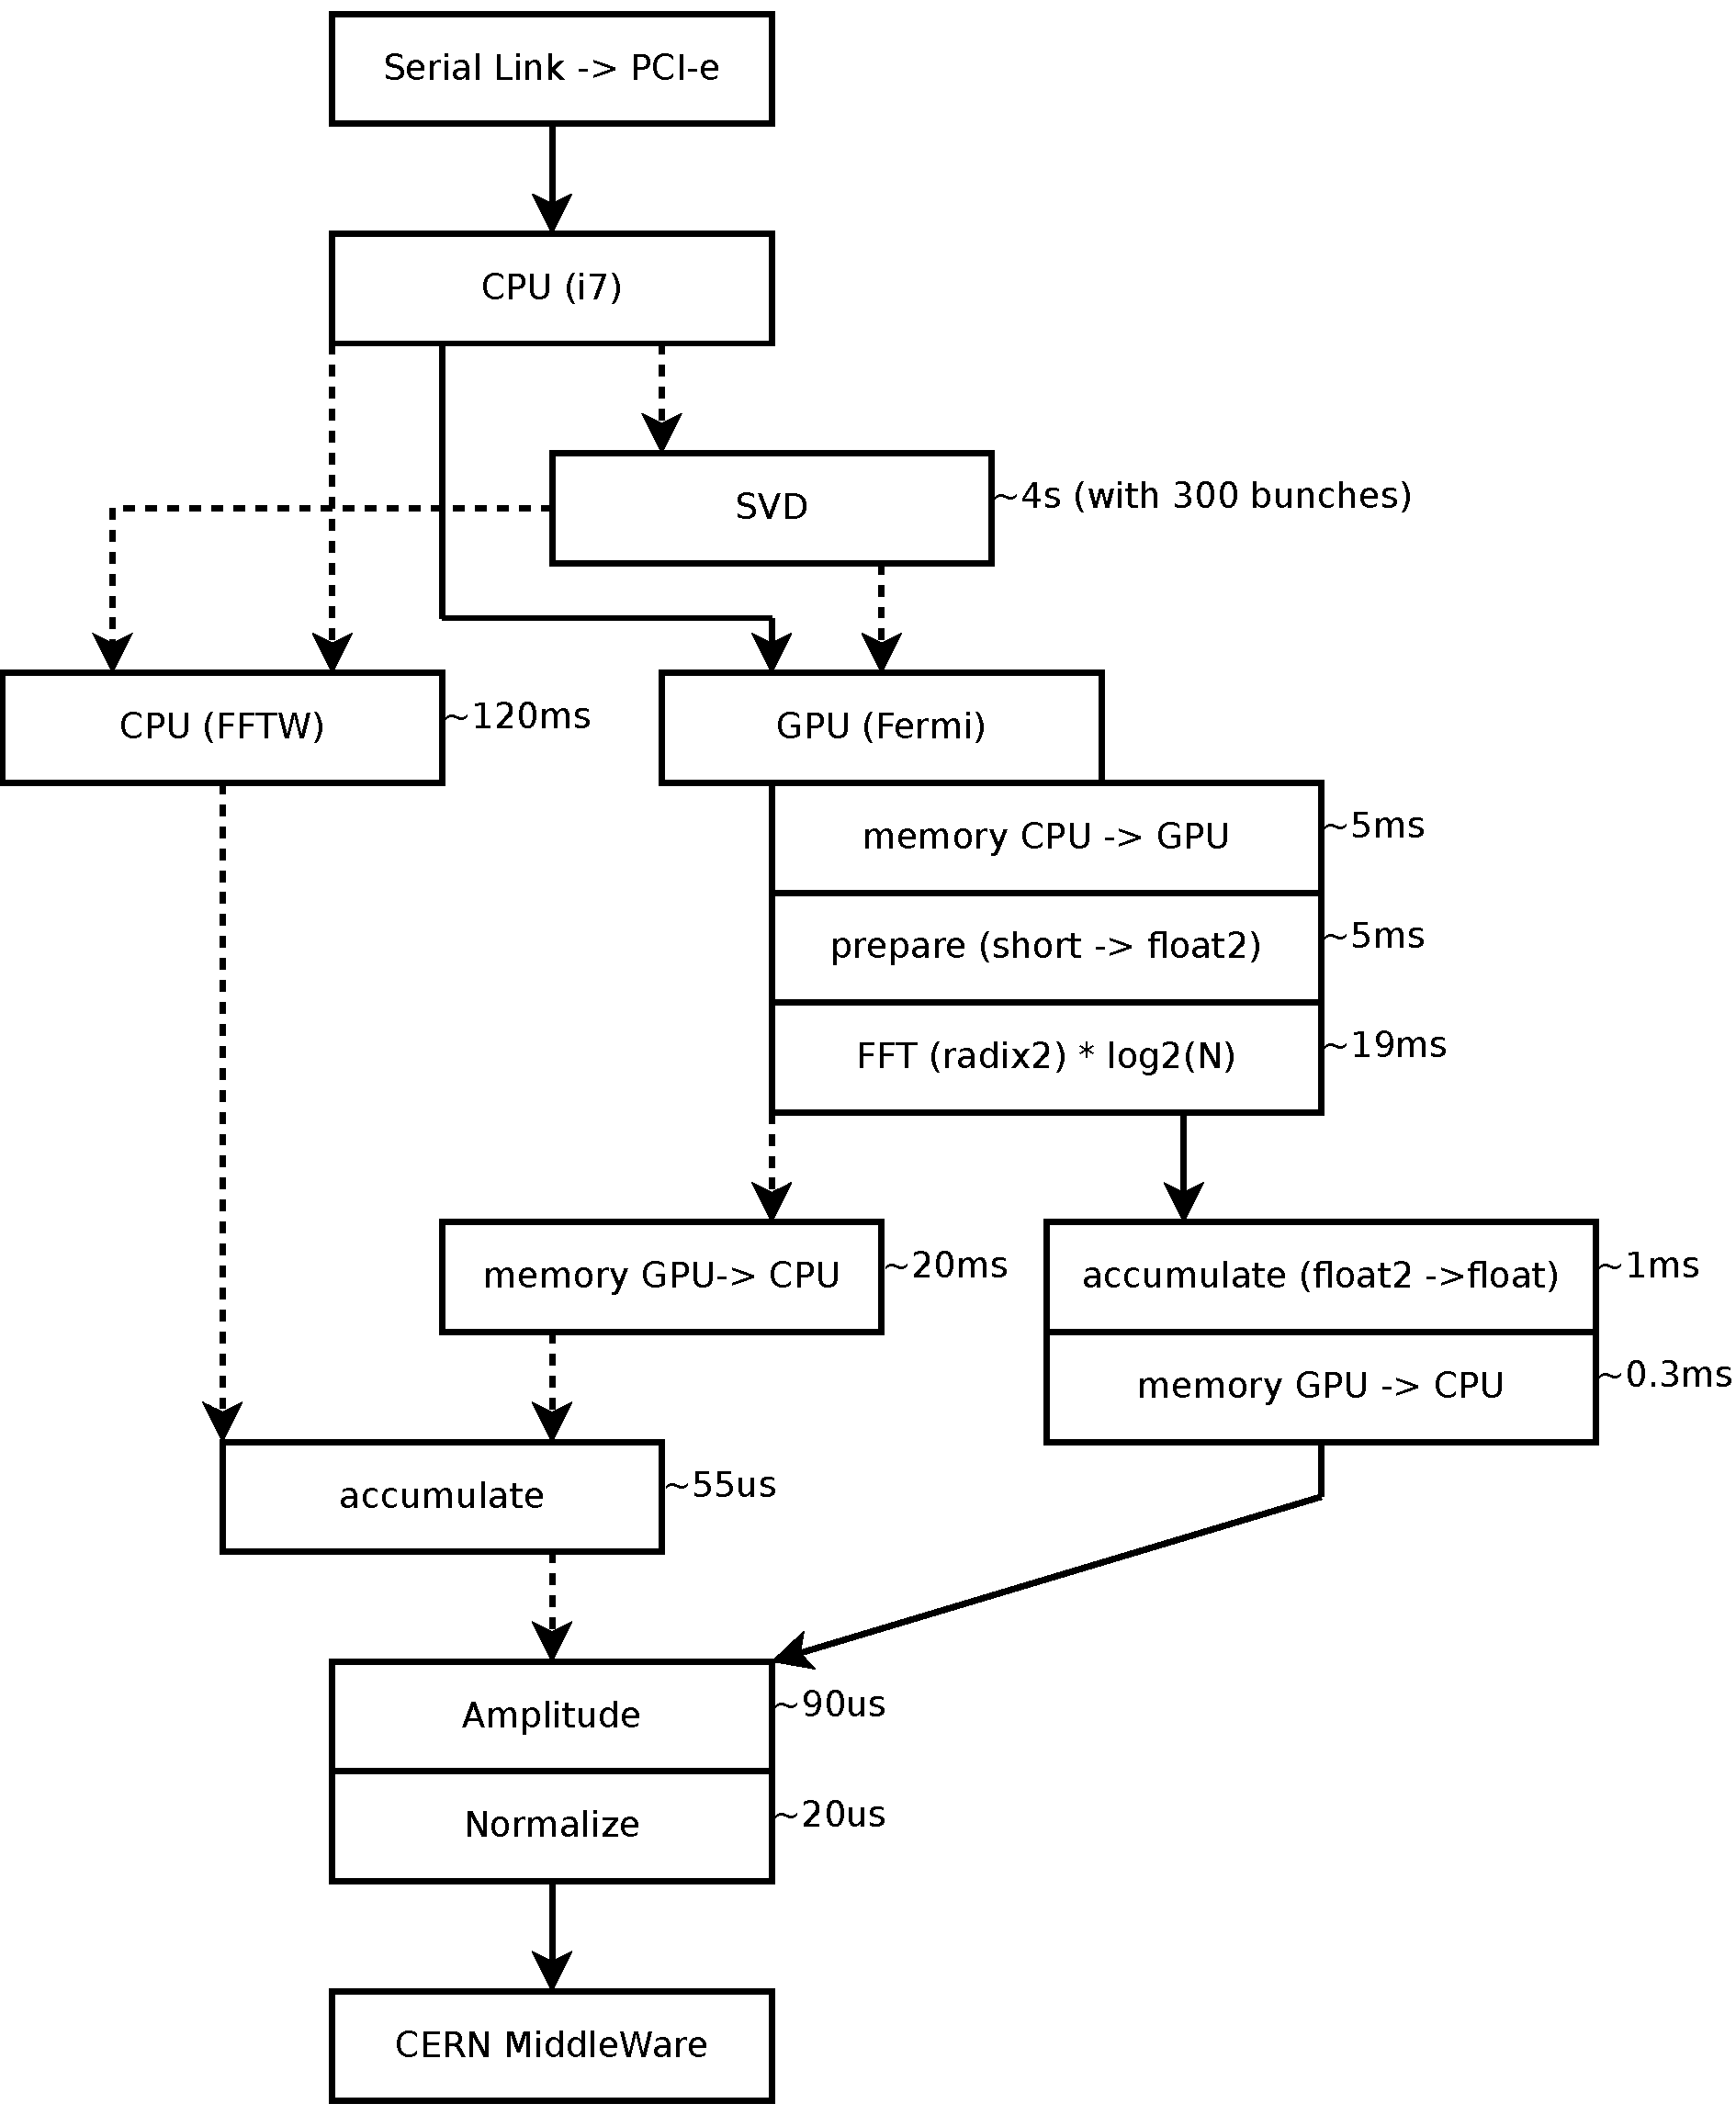
\includegraphics[scale=0.4]{PC-flow.pdf}
\end{figure}


\section{Notch filter}

Just used to cut the low frequencies this doesn't change anything on the high frequencies and was just used to allow a better imaging on the spectogram, it won't be used in the final version (quite slow because of sequencial).

\section{FFT}

Some words about FFTs.

   \subsection{FFTW}

   Some words that explain what is FFTW and why is was chosen as a reference

\begin{figure}
\caption{Spectrogram of the beam position taken on the 16 October 2012 using FFTW}
\centering
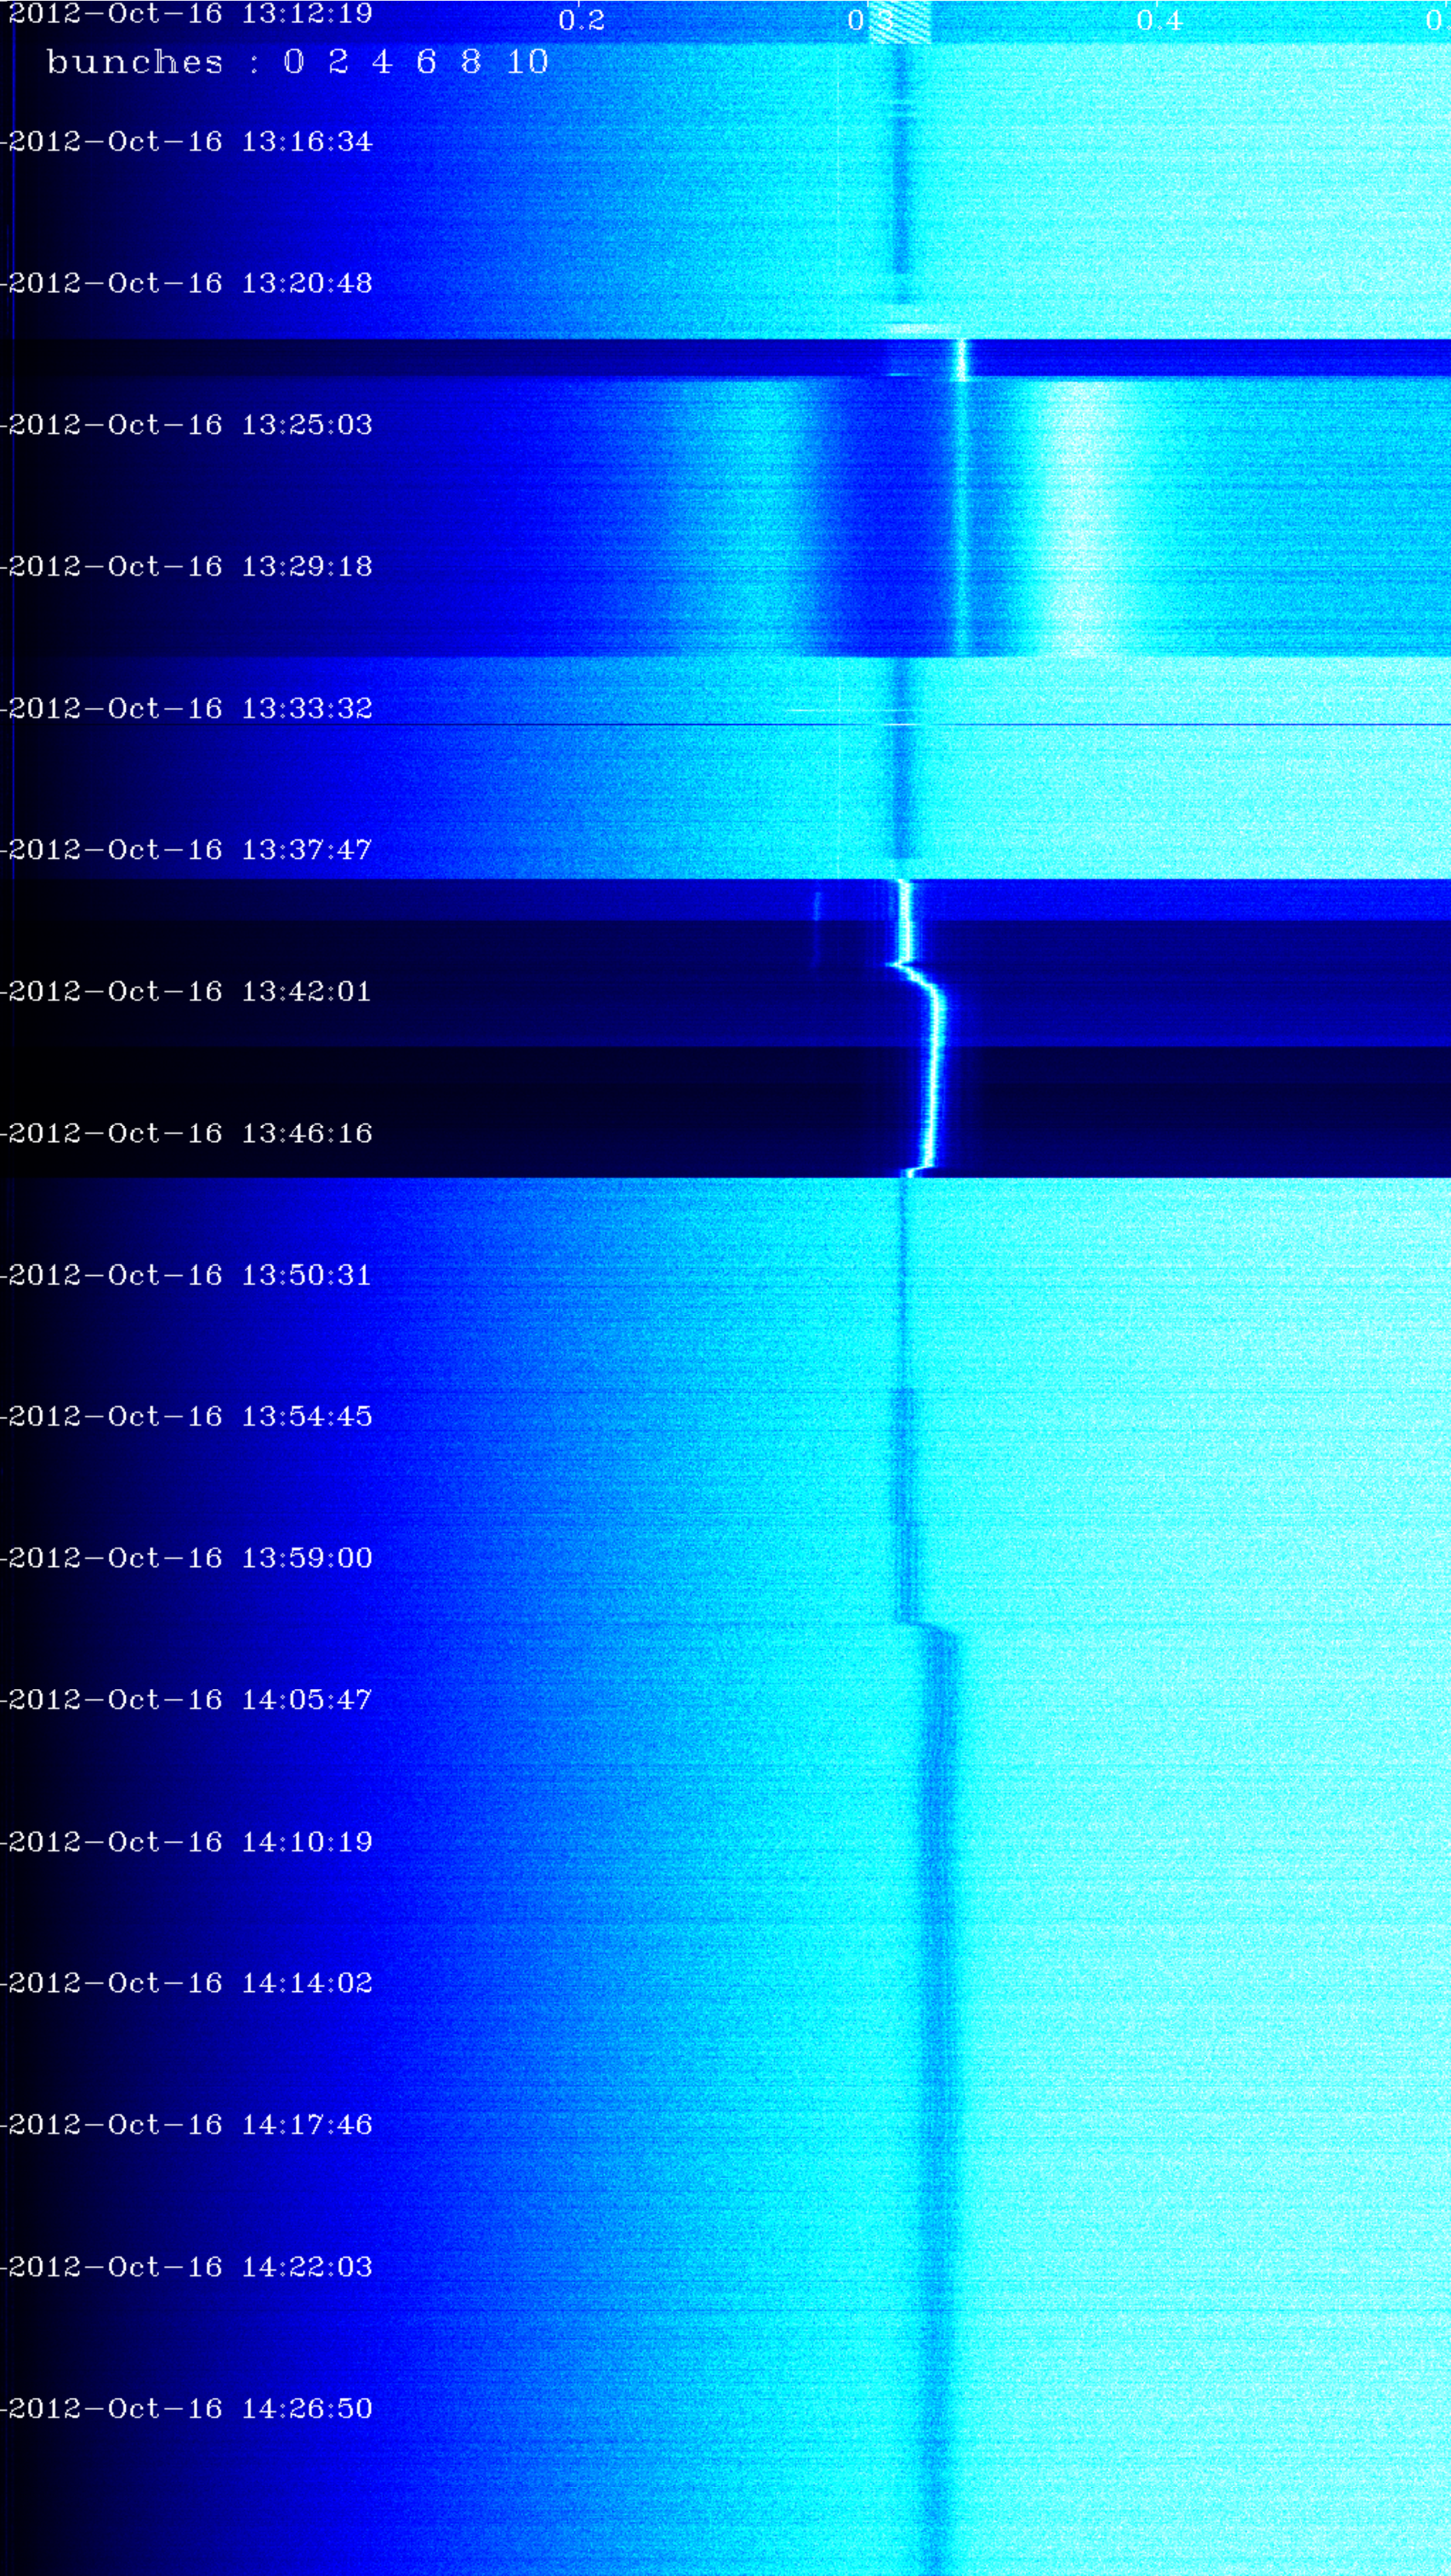
\includegraphics[scale=0.3]
{md-121016-vb1-m1-6bunches-10acc-fftw-cpu.pdf}
\end{figure}

   \subsection{FFT with OpenCL on GPU}

   Some words on the implementation used for calculating FFT on OpenCL reference to the image of the spectrogram.

\begin{figure}
\caption{Spectrogram of the beam position taken on the 16 October 2012 using OpenCL on GPU}
\centering
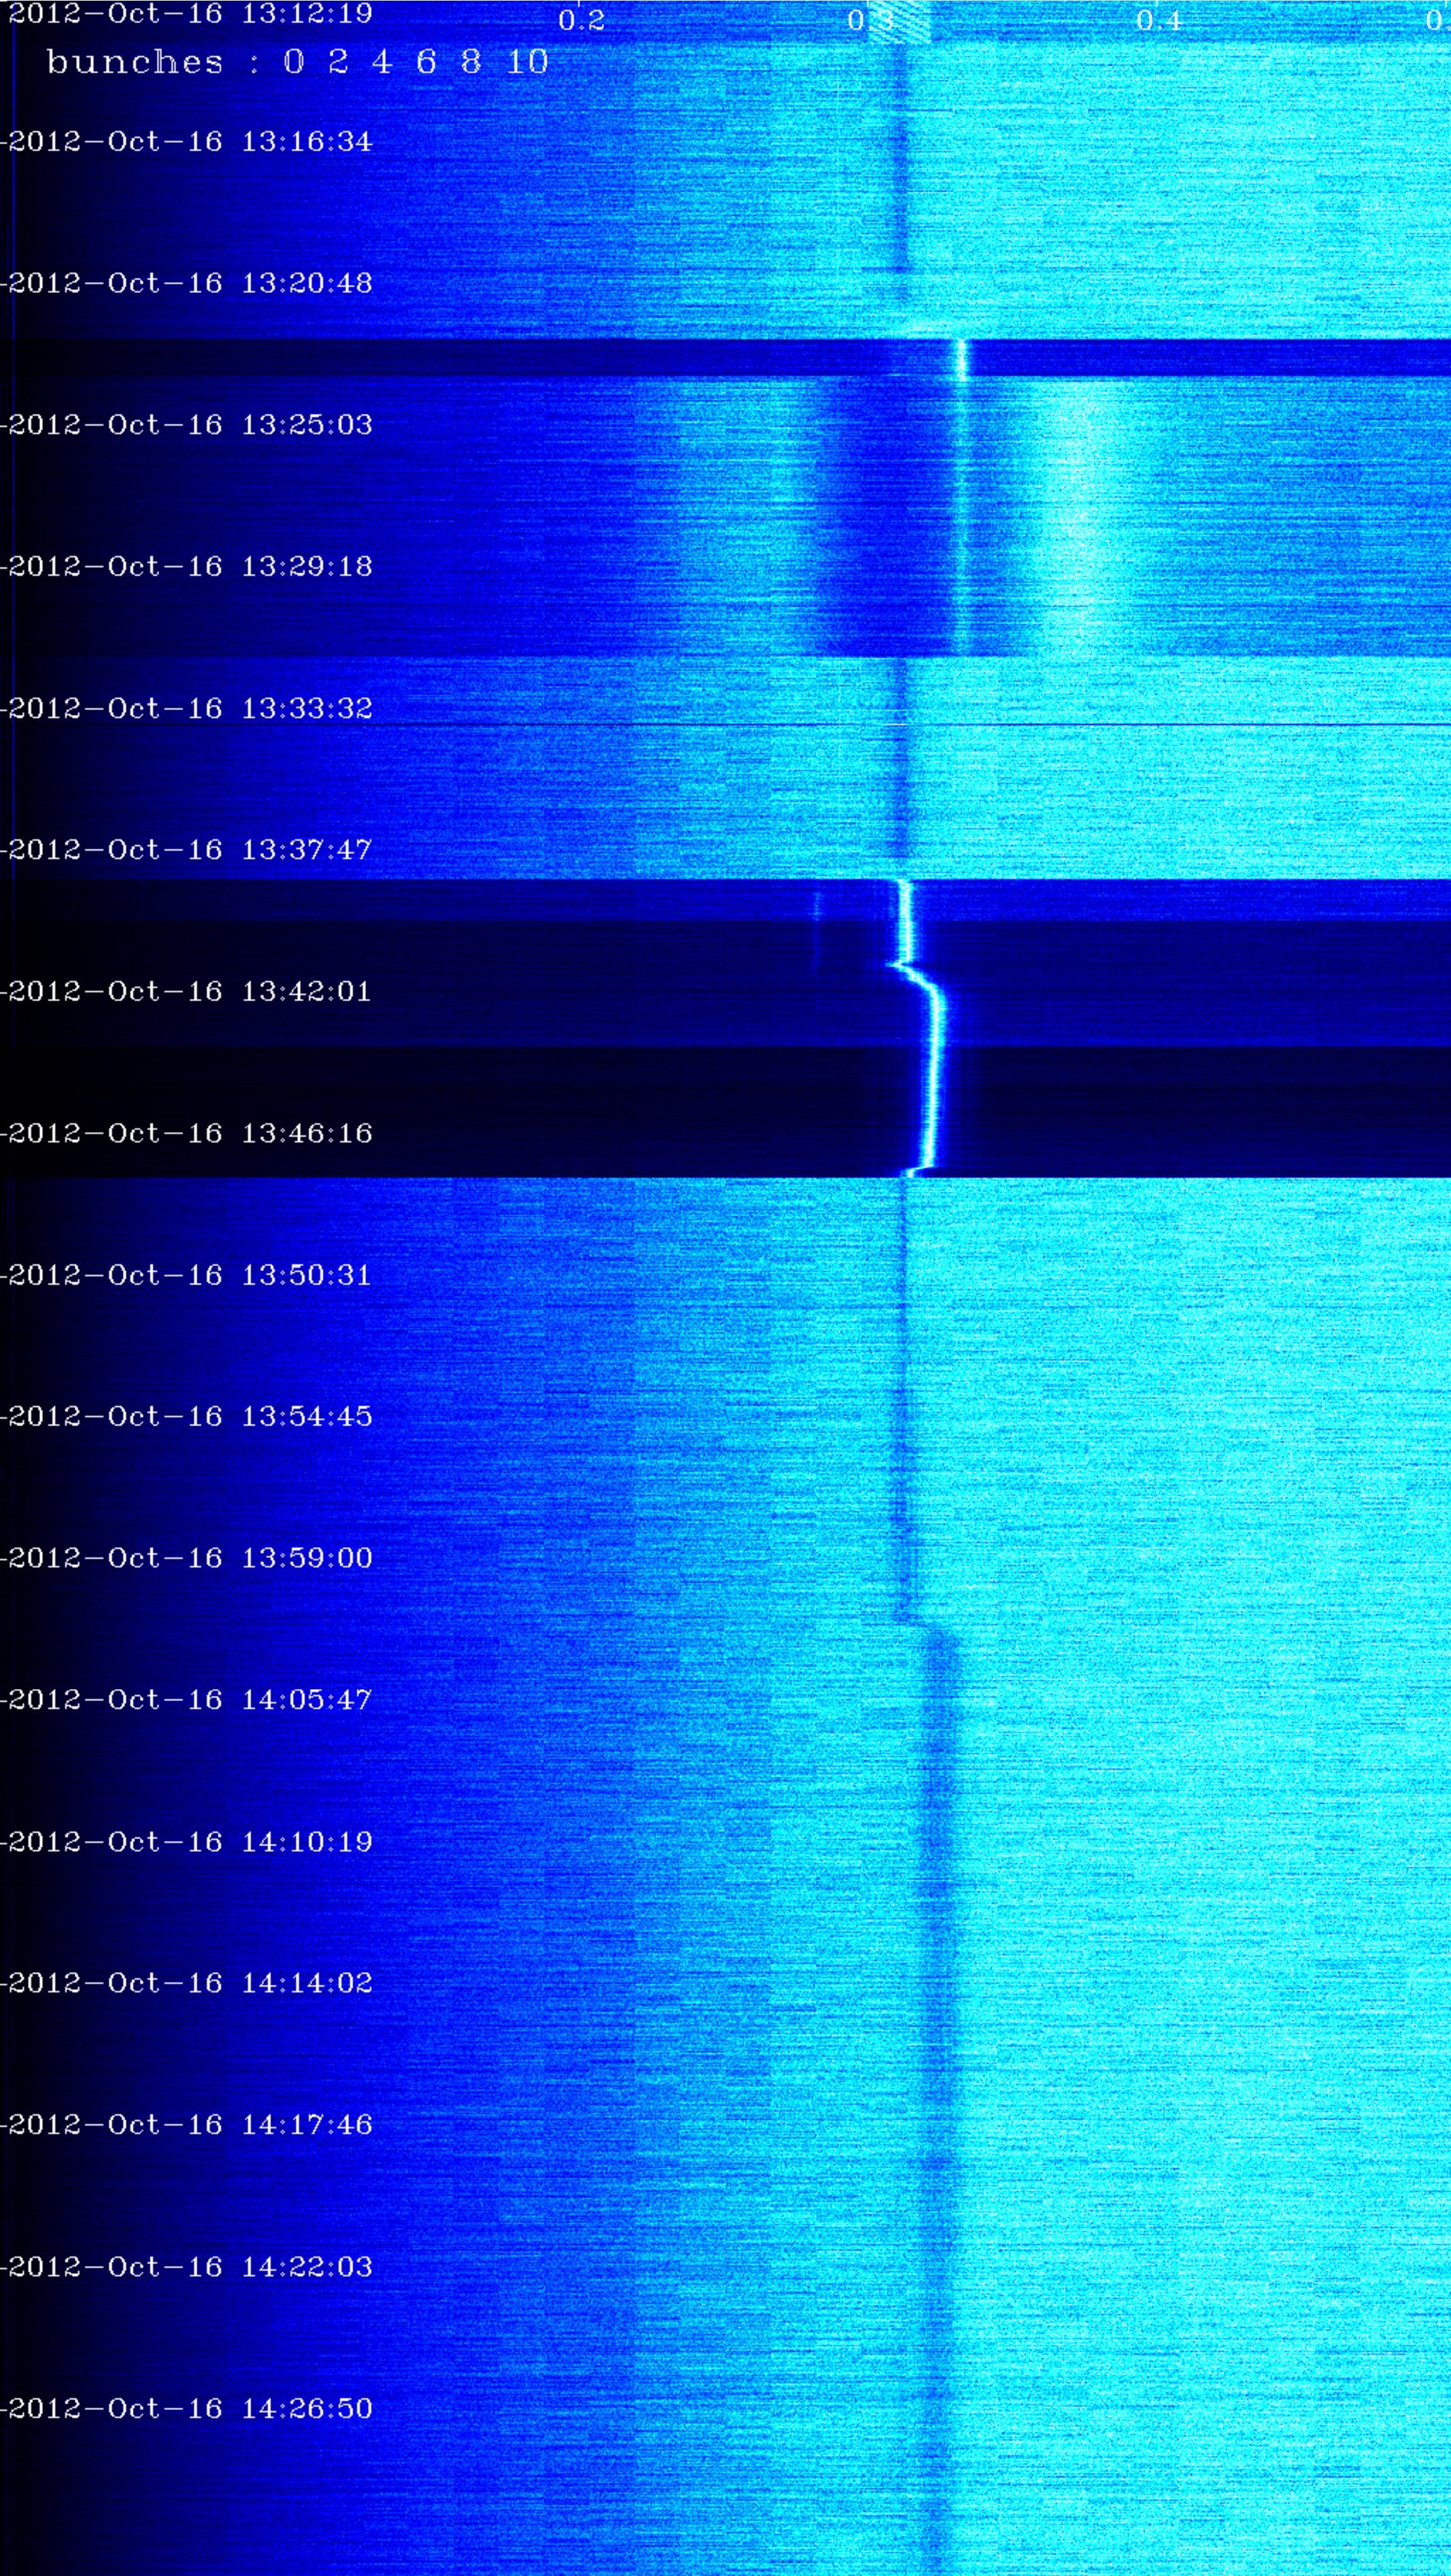
\includegraphics[scale=0.3]
{md-121016-vb1-m1-6bunches-10acc-gputopia-cl-gpu.pdf}
\end{figure}

   \subsection{FFT with OpenCL on CPU}

   Some words on the fact that you can run the code on the CPU as well and then reference on the figure.

   Also talk about the fact that there is less noise in the OpenCL CPU version than the OpenCL GPU version.

\begin{figure}
\caption{Spectrogram of the beam position taken on the 16 October 2012 using OpenCL on CPU}
\centering
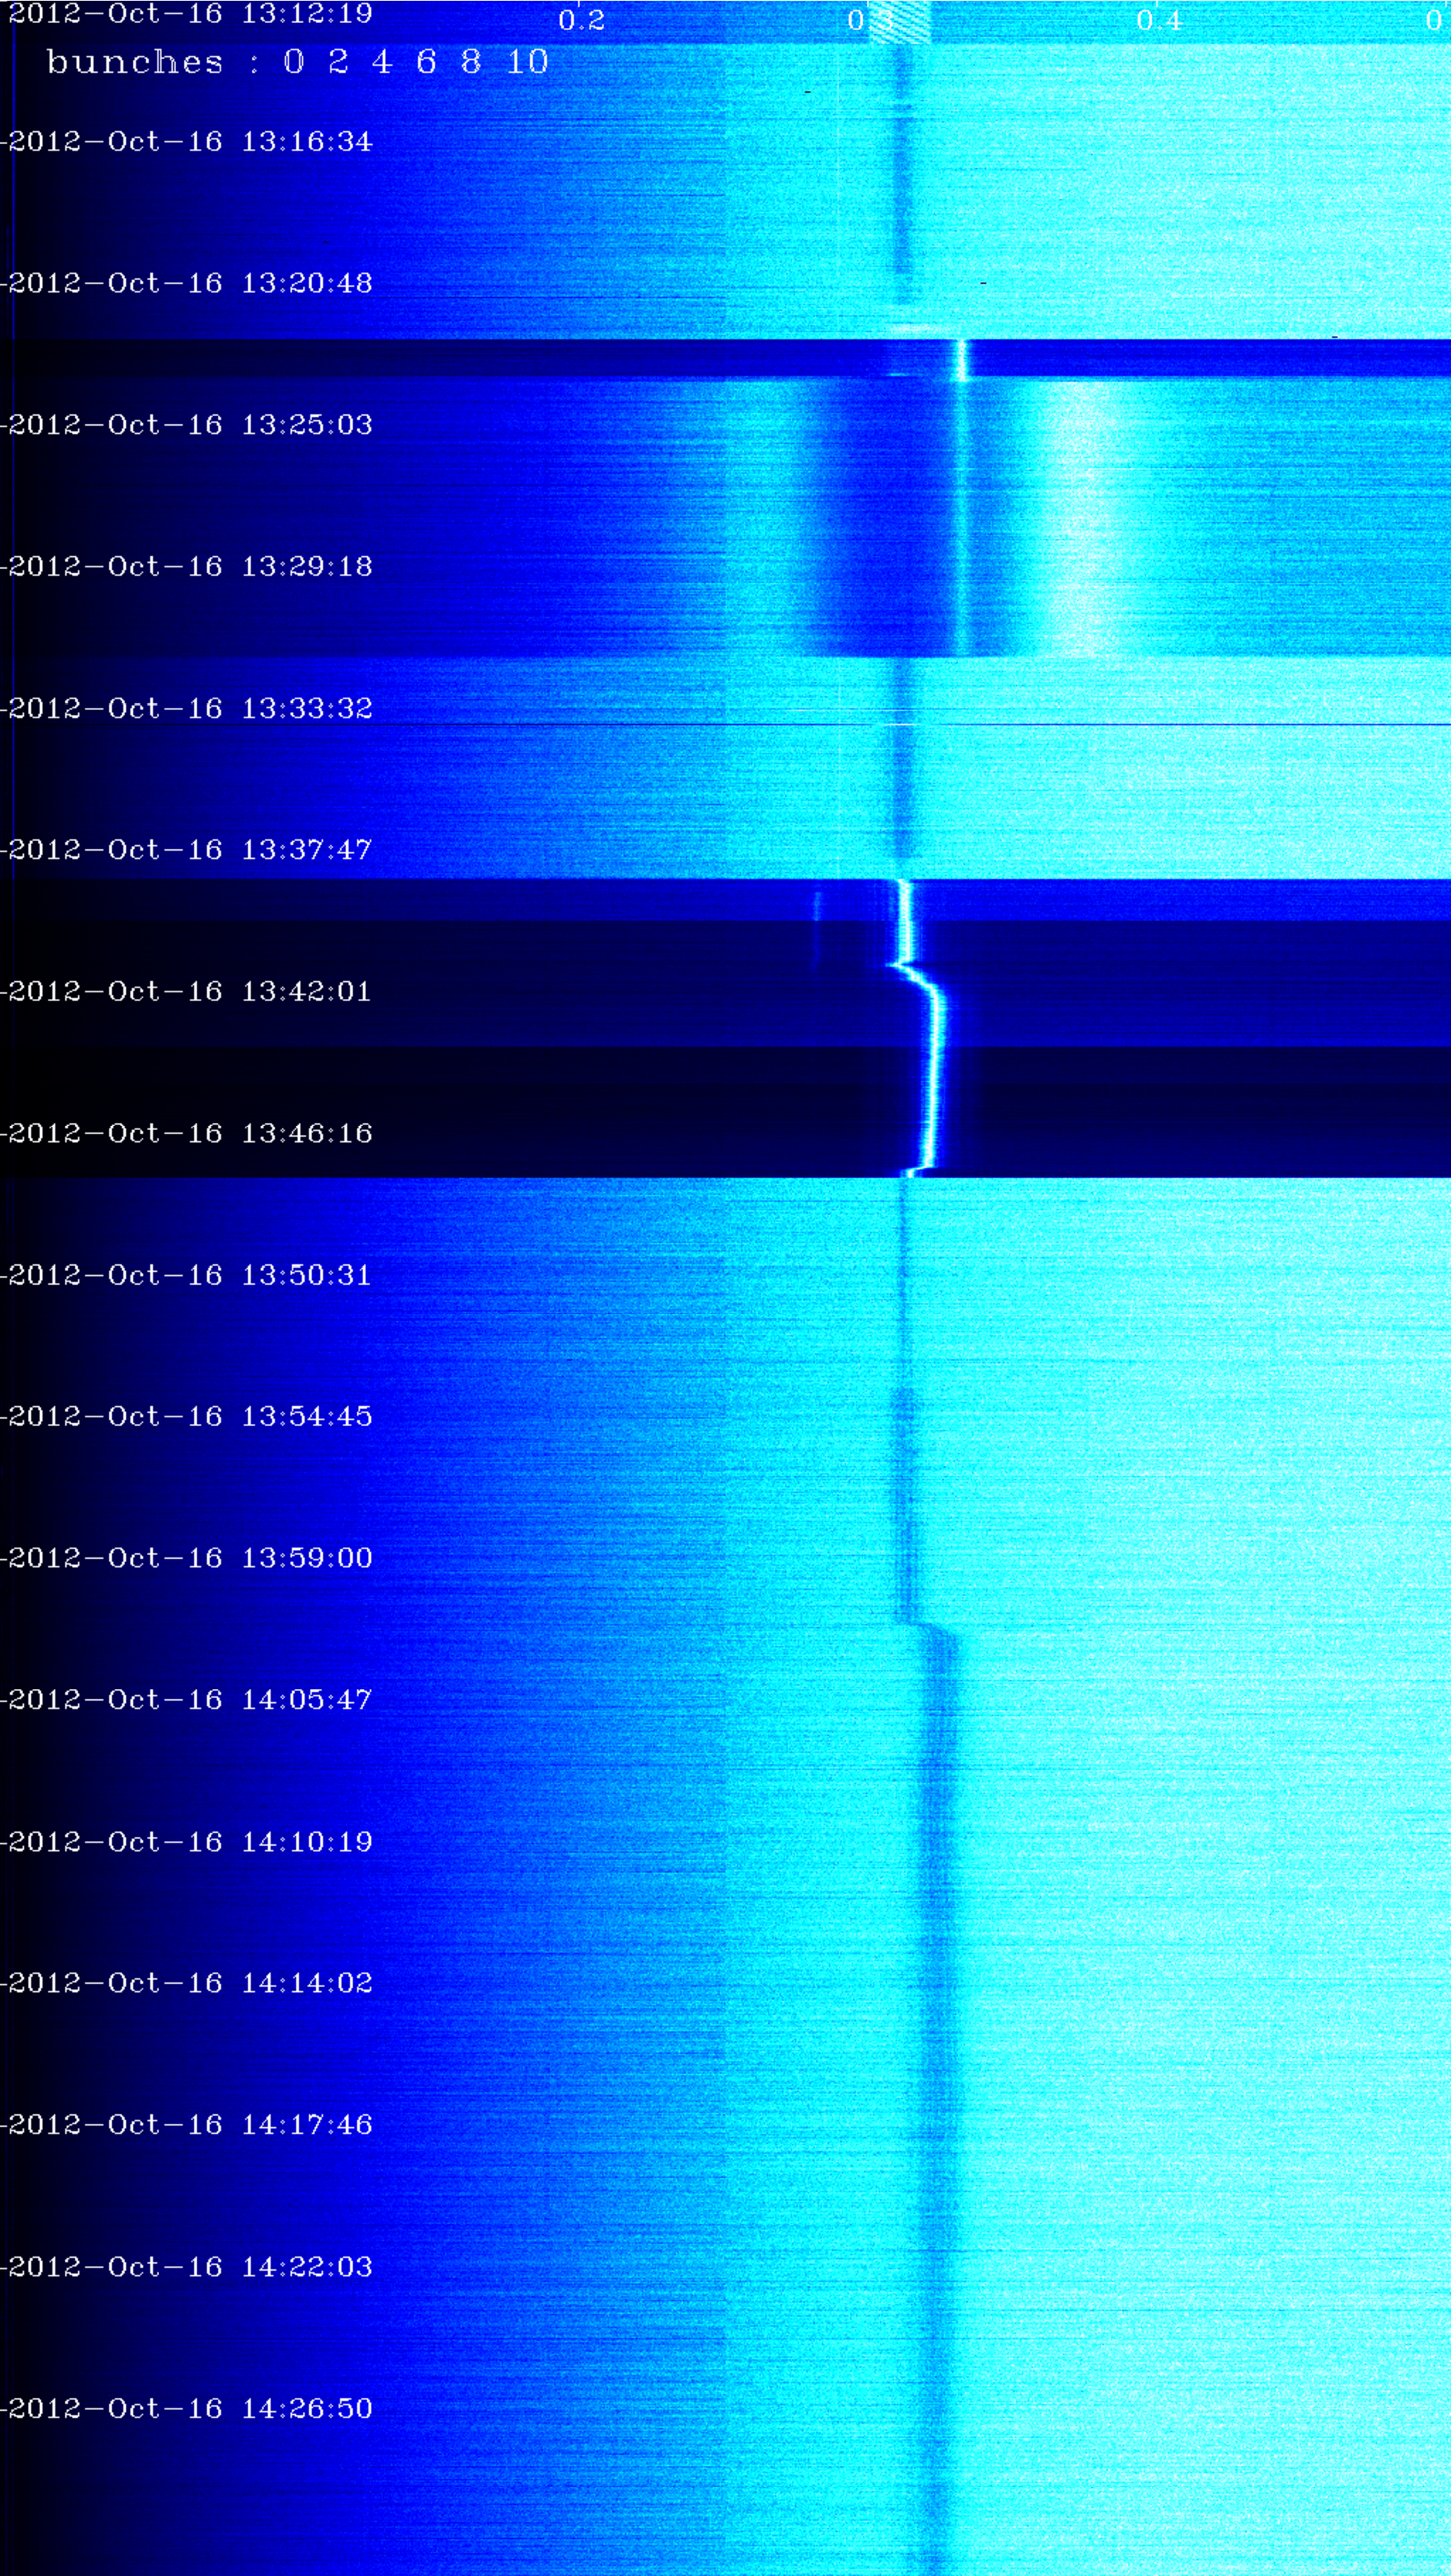
\includegraphics[scale=0.3]
{md-121016-vb1-m1-6bunches-10acc-cl-cpu-np.pdf}
\end{figure}

\section{Amplitude}

Amplitude calculation formula, explain the figures tell why it has to be done before accumulation and show this is very fast reference to the table of perf.

\section{SVD}

Problem is not direclty solvable with the number of bunch observed cite Hofle and Rama need a lot more bunches to make a good smooth\cite{calaga06}. 

Talk about the performances issues and cite the paper on SVD on GPU as a future implementation (could go to discution?)

\section{Performances}

Calculation made by accumulation to simulate the number of bunches that could be present in the final version (2880).

   \subsection{Pipelining}

	Pipelining was tested and used in the process and it was possible to win around 15\% in performances around it.

   \subsection{Memory}

	Copy of memory from and to the GPU discution.

   \subsection{Time}

	Add table with time performances and discution.